\chapter{E-commerce background} \label{chap:sota}

\section*{}

% Neste capítulo é descrito o estado da arte e são
%apresentados trabalhos relacionados para mostrar o que existe no
%mesmo domínio e quais os problemas em aberto.
%Deve deixar claro que existe uma oportunidade de desenvolvimento que
%cobre alguma falha concreta .

%O capítulo deve também efetuar uma revisão tecnológica às principais
%ferramentas utilizáveis no âmbito do projeto, justificando futuras
%escolhas.

\section{Introduction}

%Neste capítulo é ilustrada a utilização de macros \LaTeX\ para definir
%entradas no índice remissivo e são feitas diversas referências
%bibliográficas, usando-se texto de um artigo apresentado na %Conferência 
% XATA2006~\cite{kn:MVL06-xata}.

% Nos últimos tempos têm surgido diversas soluções, apresentadas por
%empresas do sector Automação de Sistemas para a disponibilização de
%sistemas \scadadms{} na \textit{Web}.

\section{Customer life cycle}

\begin{figure}[t]
  \begin{center}
    \leavevmode
    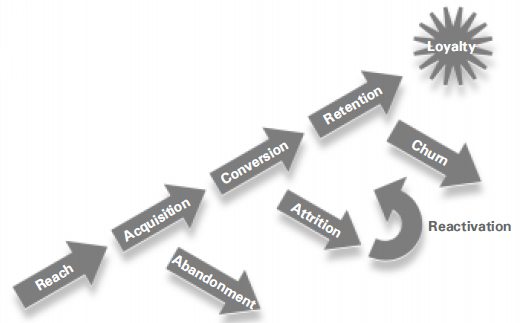
\includegraphics[width=0.86\textwidth]{lifecycle}
    \caption{Arquitectura da Solução Proposta}
    \label{fig:lifecycle}
  \end{center}
\end{figure}

Reach -> Acquisition/Abandonment -> Conversion/Attrition -> Retention / Churn -> Loyalty

\section{E-commerce metrics}

\cite{Sterne2000}

\section{Influencing user behaviour}

-> influenciar behaviour em vez de recom

\subsection{Recommendation engines}

\cite{Adomavicius2005}

\section{Summary}

No final do capítulo deverá ser apresentado um resumo com as 
principais conclusões que se podem tirar. 
